\doublespacing
%% ------------------------------------------------------------------------- %%
\chapter{Contadores de N\'{u}cleos de Condensa\c{c}\~{a}o de Nuvens}
\label{cap:CCNC_revis\~{a}o}

\PARstartOne{O}{s} CCNs, por serem muito pequenos, com uma ordem de grandeza de 10$^{-9}$ m exigem m\'{e}todos indiretos de detec\c{c}\~{a}o, sendo que a t\'{e}cnica mais utilizada ainda \'{e} a mesma que foi desenvolvida por  Wilson em 1911 para rastrear part\'{\i}culas ionizadas. Essa t\'{e}cnica, essencialmente, consiste em tornar as part\'{\i}culas opticamente detect\'{a}veis \cite{Matteo,wilson}.

Os n\'{u}cleos de condensa\c{c}\~{a}o de nuvens, quando s\~{a}o expostos a uma atmosfera supersaturada de vapor de \'{a}gua (umidade relativa maior do que 100\%), experimentam a condensa\c{c}\~{a}o desse vapor na sua superf\'{\i}cie transformando-se em  got\'{\i}culas de \'{a}gua que, por sua vez, s\~{a}o facilmente detect\'{a}veis por sensores \'{o}pticos.

Diversos contadores de CCNs (CCNC) j\'{a} foram desenvolvidos, podendo ser divididos entre os de fluxo cont\'{\i}nuo e os de fluxo est\'{a}tico, dependendo da cin\'{e}tica da parcela da atmosfera dentro do instrumento, destacando-se os CCNCs que s\~{a}o descritos a seguir: CCNC-WYO, CCNC-CFDC, CCNC-Fukuta/Saxena, CCNC-Chuang, CCNC-Peter e CCNC-MPI-Chemie.

%% ------------------------------------------------------------------------- %%

\section{CCNC-WYO}

O CCNC-WYO foi desenvolvido no Departamento de Ci\^{e}ncias da Atmosfera da Universidade do Wyoming - EUA.
Estruturado na c\^{a}mara de nuvens de difus\~{a}o t\'{e}rmica est\'{a}tica de placas paralelas, este equipamento \'{e} utilizado h\'{a} d\'{e}cadas.

Langsdorf, em 1939 \cite{Langsdorf} apresentou \`{a} comunidade cient\'{\i}fica uma vers\~{a}o dessa tecnologia de c\^{a}mara com a finalidade de detectar part\'{\i}culas ionizadas e esta tecnologia obedece ao mesmo princ\'{\i}pio da C\^{a}mara de Wilson. Entretanto, \'{e} Twomey \cite{twomey} que adapta essa c\^{a}mara para a medida da concentra\c{c}\~{a}o dos CCNs.

 O princ\'{\i}pio de funcionamento desse equipamento consiste em criar uma regi\~{a}o de press\~{a}o parcial de vapor $P_v$ maior do que a press\~{a}o de satura\c{c}\~{a}o de vapor d'agua $P_{sv}$, na regi\~{a}o central da c\^{a}mara de nuvens, ou seja, uma umidade relativa, $UR=(P_v/P_{sv}) \cdot 100\%$, maior do que 100\% nessa regi\~{a}o. A press\~{a}o de satura\c{c}\~{a}o de vapor d'agua \'{e} a press\~{a}o em que o vapor se liquefaz em condi\c{c}\~{o}es ideais, sendo uma propriedade que depende da temperatura de forma n\~{a}o linear \cite{wagner}. Nessa condi\c{c}\~{a}o de supersatura\c{c}\~{a}o positiva, $S=UR-100\%$, got\'{\i}culas se originam a partir da condensa\c{c}\~{a}o do vapor de \'{a}gua na superf\'{\i}cie dos CCNs presentes na c\^{a}mara. Esse processo ocorre naturalmente na natureza e \'{e} chamado de nuclea\c{c}\~{a}o heterog\^{e}nea. Nessa situa\c{c}\~{a}o se diz que os CCNs est\~{a}o ativados.

 O valor da supersatura\c{c}\~{a}o, dentro da c\^{a}mara de nuvens, n\~{a}o \'{e} a mesma ao longo da sua altura $z$. A condi\c{c}\~{a}o de supersatura\c{c}\~{a}o m\'{a}xima, ocorre aproximadamente a meia altura da c\^{a}mara e \'{e} obtida atrav\'{e}s da difus\~{a}o de umidade, a partir das duas placas mantidas em diferentes temperaturas.

Os perfis estimados de temperatura $T$, press\~{a}o parcial de vapor $P_v$, de satura\c{c}\~{a}o de vapor $P_{sv}$ e de supersatura\c{c}\~{a}o $S$ na c\^{a}mara de nuvens est\~{a}o mostrados na Figura \ref{perfil} e s\~{a}o calculados pelas seguintes express\~{o}es \cite{wagner,Frank}:


\begin{equation}
\label{eq01}
s(z)  = \frac{{P_v(z) }}{{P_{sv} }} \cdot 100 - 100,
\end{equation}

\begin{equation}
\label{eq02}
P_v(z)  = \frac{{P_{sv}(T_s )  - P_{sv}(T_i ) }}{H}z + P_{sv}(T_i ),
\end{equation}

\begin{equation}
\label{eq03}
P_{sv}(T)  = 0,61078\exp \left( {\frac{{17,269T}}{{T + 237,3}}} \right),
\end{equation}

\begin{equation}
\label{eq04}
T(z)  = \frac{{T_s  - T_i }}{H}z + T_i,
\end{equation}

\begin{flushleft} em que: $P_{v}(z)$ \'{e} a press\~{a}o parcial de vapor de \'{a}gua na altura $z$;
$P_{sv}(T)$ \'{e} a press\~{a}o de satura\c{c}\~{a}o de vapor;
$H$ \'{e} a altura da SDCC;
$T_{s}$ ,$T_{i}$  s\~{a}o respectivamente as temperaturas das tampas superior e inferior da c\^{a}mara de nuvens e
$T(z)$ \'{e} a temperatura na altura $z$.
\end{flushleft}

\begin{figure}[hbt]
\begin{center}
%\includegraphics[scale=0.9]{eps/supersaturacao_na_SDTC3.eps}\\
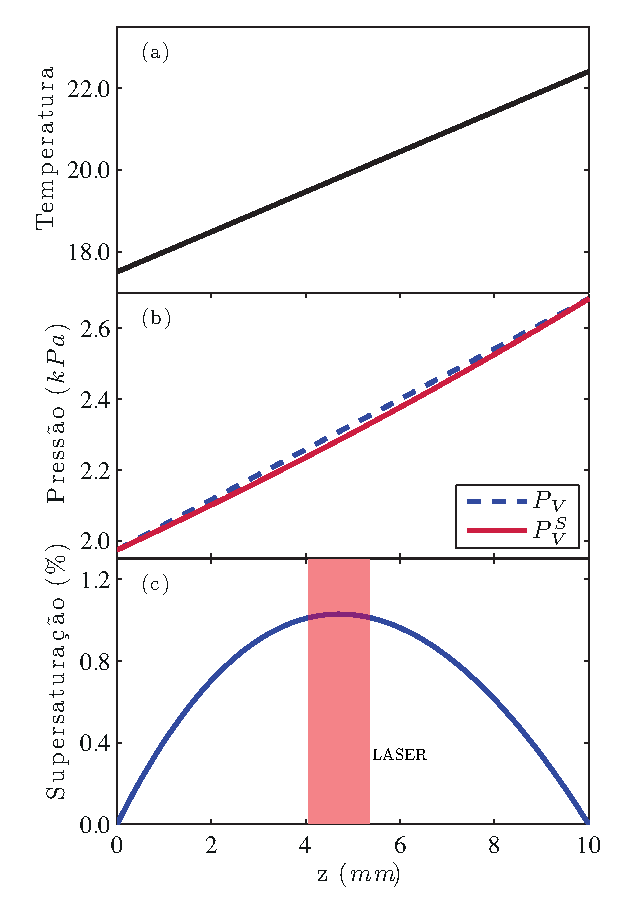
\includegraphics[scale=0.8]{eps/figSaturacao.eps}\\
\end{center}
\caption{\label{perfil}\hspace{-0.1em} perfil vertical de temperatura, (a) press\~{a}o; (b) de supersatura\c{c}\~{a}o; (c) dentro da c\^{a}mara de nuvens.}
\end{figure}



%\begin{figure}[htb]
%\begin{center}
%\includegraphics[scale=1.0]{eps/CCNC_WYO.eps}\\
%\end{center}
%\caption{\label{CCNCSDCC}\hspace{-0.1em} Diagrama esquem\'{a}tico do CCNC-WYO,  (a)  vista superior da c\^{a}mara de %nuvens; (b) vista lateral.}
%\end{figure}





Os perfis, mostrados na Figura \ref{perfil},  foram calculados considerando-se a temperatura da placa superior $T_s$ de 22,37$^o$C e a temperatura da placa inferior $T_i$ de 17,51$^o$C. Os gradientes constantes de temperatura e press\~{a}o (Figura \ref{perfil} a e b) s\~{a}o presumidos a partir dos valores de temperatura medidos nas placas inferior e superior da c\^{a}mara de nuvens e partem da suposi\c{c}\~{a}o de que a press\~{a}o parcial de vapor nas regi\~{o}es imediatamente pr\'{o}ximas \`{a}s placas \'{e} igual a press\~{a}o de satura\c{c}\~{a}o para as respectivas temperaturas.

Percebe-se na Figura \ref{perfil} (c) que a curva de supersatura\c{c}\~{a}o dentro da c\^{a}mara de nuvens, derivada a partir de $P_v$ e $P_{sv}$, possui um perfil aproximadamente parab\'{o}lico com o m\'{a}ximo \`{a} meia altura da c\^{a}mara. Essa altura $z$, onde a supersatura\c{c}\~{a}o \'{e} m\'{a}xima, \'{e} a regi\~{a}o de interesse para an\'{a}lise, pois, \'{e} nessa regi\~{a}o onde o maior n\'{u}mero de CCNs presentes na c\^{a}mara s\~{a}o ativados. Assim sendo, um feixe cil\'{\i}ndrico de luz LASER ilumina as got\'{\i}culas formadas nessa regi\~{a}o, permitindo a sua detec\c{c}\~{a}o por sensores \'{o}pticos. No caso do CCNC-WYO, o valor da concentra\c{c}\~{a}o de CCNs \'{e} obtido a partir da medi\c{c}\~{a}o da intensidade da luz espalhada pelas got\'{\i}culas ao atravessar a luz LASER.

As t\'{e}cnicas de espalhamento s\~{a}o largamente empregadas em medi\c{c}\~{o}es indiretas de fen\^{o}menos atmosf\'{e}ricos tais como nuvens formadas por got\'{\i}culas de \'{a}gua \cite{Frisvad}. No caso das medi\c{c}\~{o}es dos CCNs, estas s\~{a}o baseadas na exist\^{e}ncia de uma rela\c{c}\~{a}o entre a concentra\c{c}\~{a}o de got\'{\i}culas (part\'{\i}culas) e a intensidade da luz espalhada quando estas s\~{a}o iluminadas por um feixe de luz. Essa rela\c{c}\~{a}o, entretanto, \'{e}  complexa, tornando-se necess\'{a}ria a utiliza\c{c}\~{a}o de equa\c{c}\~{o}es emp\'{\i}ricas com coeficientes a serem determinados experimentalmente \cite{Oliveira} a partir da an\'{a}lise visual de fotografias. Al\'{e}m disso, essa metodologia introduz incertezas intr\'{\i}nsecas associadas ao fato de que o espalhamento de luz depende n\~{a}o somente da concentra\c{c}\~{a}o das part\'{\i}culas, mas tamb\'{e}m das "se\c{c}\~{o}es de choque" e, portanto, da geometria de cada part\'{\i}cula no caminho do feixe \cite{Oliveira}. A distribui\c{c}\~{a}o angular do espalhamento da luz pode ser rigorosamente determinada em condi\c{c}\~{o}es controladas \cite{McMurry}. Entretanto, este n\~{a}o \'{e} o caso das medi\c{c}\~{o}es dos CCNs na atmosfera, onde as caracter\'{\i}sticas f\'{\i}sicas e qu\'{\i}micas das part\'{\i}culas s\~{a}o imprevis\'{\i}veis. Outra quest\~{a}o importante \'{e} o ru\'{\i}do intr\'{\i}nseco  ao sistema eletr\^{o}nico de fotodetec\c{c}\~{a}o, nas suas mais diversas formas (t\'{e}rmico e/ou induzido),  que deteriora a rela\c{c}\~{a}o sinal ru\'{\i}do, principalmente em situa\c{c}\~{o}es de baixa concentra\c{c}\~{a}o \cite{Pinheiro}.

O CCNC-WYO \'{e} constitu\'{\i}do por um cilindro de 10,0 cm de di\^{a}metro e 1,0 cm de altura, de parede lateral feita de material isolante t\'{e}rmico e imperme\'{a}vel. O gradiente de temperatura, necess\'{a}rio para se obter uma determinada supersatura\c{c}\~{a}o, \'{e} obtido a partir do controle da diferen\c{c}a de temperatura entre placas de alum\'{\i}nio que fecham as extremidades inferior e superior da cavidade cil\'{\i}ndrica. A placa inferior \'{e} acoplada a dois resfriadores est\'{a}ticos (pastilhas Peltier) e o gradiente desejado \'{e} mantido atrav\'{e}s de um controlador de temperatura do tipo proporcional, integral e diferencial (PID). Pap\'{e}is absorventes, aderidos nas placas de alum\'{\i}nio, s\~{a}o abastecidos por um reservat\'{o}rio de \'{a}gua destilada, mantendo uma umidade igualmente distribu\'{\i}da. O ar com os aeross\'{o}is que se deseja quantificar \'{e} admitido na c\^{a}mara atrav\'{e}s do acionamento de uma bomba. Posteriormente \`{a} desativa\c{c}\~{a}o da bomba a c\^{a}mara de nuvens \'{e} selada. Nesse momento, ocorre um transit\'{o}rio de ativa\c{c}\~{a}o de CCNs que deve ser descartado, at\'{e} que o sistema entre em equil\'{\i}brio e se inicie o processo de ativa\c{c}\~{a}o dos CCNs na supersatura\c{c}\~{a}o desejada.

O processo de ativa\c{c}\~{a}o dos CCNs \'{e}, portanto, um processo din\^{a}mico e a concentra\c{c}\~{a}o na regi\~{a}o de interesse cresce rapidamente, at\'{e} que todos os CCNs estejam ativados. Ap\'{o}s este processo este n\'{u}mero cai gradativamente, devido \`{a} a\c{c}\~{a}o da gravidade.

O diagrama esquem\'{a}tico do CCNC-WYO \'{e} apresentado na Figura \ref{CCNCSDCC}. Na parte superior (a), destacam-se a vista superior da c\^{a}mara de nuvens, uma fonte de luz LASER (635 nm), fotodetector para medi\c{c}\~{a}o de luz espalhada al\'{e}m da bomba, v\'{a}lvulas e controlador que comanda a entrada de ar atmosf\'{e}rico para o interior da c\^{a}mara de nuvens. Na parte inferior (b), destacam-se a vista lateral da c\^{a}mara de nuvens, o posicionamento das pastilhas Peltier, o papel saturado com \'{a}gua, os sensores de temperatura, o controlador PID de temperatura e o reservat\'{o}rio de \'{a}gua.



\begin{figure}[htb]
\begin{center}
\includegraphics[scale=1.0]{eps/CCNC_WYO.eps}\\
\end{center}
\caption{\label{CCNCSDCC}\hspace{-0.1em} diagrama esquem\'{a}tico do CCNC-WYO,  (a)  vista superior da c\^{a}mara de nuvens; (b) vista lateral.}
\end{figure}


%% ------------------------------------------------------------------------- %%


\section{CCNC-CFDC}

O CCNC-CFDC (\textit{Continuous Flow Parallel Plate Thermal Diffusion Chamber}) \'{e} baseado na c\^{a}mara de difus\~{a}o de placas paralelas mas de fluxo cont\'{\i}nuo \cite{Sinnarwalla} e foi desenvolvido para
superar as limita\c{c}\~{o}es e defici\^{e}ncias do CCNC do tipo est\'{a}tico. Pelo fato dessa alternativa de
instrumento operar de modo cont\'{\i}nuo, os efeitos transit\'{o}rios,
provocados pela abertura e fechamento de v\'{a}lvulas comuns na c\^{a}mara de nuvens,
n\~{a}o ocorrem. Isto favorece uma medi\c{c}\~{a}o cont\'{\i}nua da concentra\c{c}\~{a}o de CCNs, ao mesmo tempo que, por sua vez, melhora a resolu\c{c}\~{a}o temporal. Al\'{e}m disto, como a amostra \'{e} confinada no eixo axial
da c\^{a}mara, todo os CCNs s\~{a}o expostos ao mesmo valor de supersatura\c{c}\~{a}o. No
que diz respeito ao limite inferior de  supersatura\c{c}\~{a}o,  este deve
ficar acima de 0,1\% pois, abaixo deste valor, uma gota de nuvem precisa
de um tempo maior do que aquele dispon\'{\i}vel para sua passagem (queda) pela regi\~{a}o (cilindro) de amostragem.

Na CFDC suas placas paralelas podem ser dispostas tanto na horizontal quanto na vertical. Quando as placas est\~{a}o dispostas na horizontal, a queda de gotas, pela a\c{c}\~{a}o do campo gravitacional, limita
o tempo durante o qual as gotas experimentam uma supersatura\c{c}\~{a}o uniforme.


Na Figura \ref{cfcd} \'{e} apresento um diagrama esquem\'{a}tico da c\^{a}mara do CCNC-CFDC cujas dimens\~{o}es s\~{a}o $ 100\ \ cm$ x $13,2\ \ cm$,  sendo que o di\^{a}metro  interno \'{e} de $1,0\ \ cm$.

%No caso nas placas orientadas na vertical, conforme mostrado na Figura \ref{cfcd}, existe um limite relacionado \`{a} diferen\c{c}a de temperatura m\'{a}xima, pois, um alto valor para este par\^{a}metro induz um fluxo de empuxo.

A id\'{e}ia b\'{a}sica do CCNC-CFDC  \'{e} expor um dado aerosol a um campo vari\'{a}vel de supersatura\c{c}\~{a}o
e inferir o espectro dos CCNs pela distribui\c{c}\~{a}o de tamanho de gotas em
sua sa\'{\i}da. Os CCNs com baixa supersatura\c{c}\~{a}o cr\'{\i}tica s\~{a}o ativados, isto \'{e},
iniciam o processo de crescimento, numa regi\~{a}o pr\'{o}xima da entrada da c\^{a}mara de difus\~{a}o. Portanto, estes t\^{e}m mais tempo para crescer do que aqueles que possuem um alto valor de supersatura\c{c}\~{a}o
cr\'{\i}tica.

O sistema de medida da concentra\c{c}\~{a}o no CCNC-CFDC \'{e} baseado no espalhamento de luz. Dessa forma, os problemas relativos \`{a} calibra\c{c}\~{a}o apresentados pelo CCNC-WYO tamb\'{e}m est\~{a}o presentes nessa tecnologia.

\begin{figure}[!hbt]
\begin{center}
\includegraphics[scale=0.80]{eps/cfcd.eps}\\
\end{center}
\caption{\label{cfcd}\hspace{-0.1em} diagrama esquem\'{a}tico da c\^{a}mara do CCNC-CFDC.}
\end{figure}


\section{CCNC-FUKUTA/SAXENA}
Fukuta e Saxena \cite{Fukuta2} propuseram uma modifica\c{c}\~{a}o na CFDC. Nessa proposta, um gradiente
de temperatura \'{e} gerado de forma perpendicular ao fluxo de CCNs. Isto faz com que as part\'{\i}culas, com o mesmo tempo de exposi\c{c}\~{a}o dentro da c\^{a}mara,
experimentem diferentes supersatura\c{c}\~{o}es numa faixa de 0,15\% a 1,2\%. Assim, este
instrumento pode ser visto como um conjunto de CFDC com differentes
temperaturas entre as placas, operando de forma paralela.

O CCNC-FUKUTA/SAXENA utiliza um sensor \'{o}ptico da Climent Instruments modelo CI201
que, na realidade, \'{e} um analisador de part\'{\i}culas por n\'{\i}vel de tens\~{a}o
de pulso. Assim sendo, como nos demais instrumentos que n\~{a}o usam
processamento digital de imagens, ou que n\~{a}o possuem mecanismos de
fotografia para posterior contagem manual, um procedimento de
calibra\c{c}\~{a}o baseado na gera\c{c}\~{a}o de aeross\'{o}is mono-dispersivos de
concentra\c{c}\~{o}es conhecidas, se faz necess\'{a}rio.

Apesar do CCNC-FUKUTA/SAXENA apresentar uma evolu\c{c}\~{a}o significativa em rela\c{c}\~{a}o aos CCNCs anteriores, as dimens\~{o}es da c\^{a}mara de condensa\c{c}\~{a}o ($83,8\ \ cm$ $\times$ $1,8\ \ cm$ $\times$ $19,1\ \ cm$) e o seu peso maior ($26\ \ Kg$) inviabilizam sua utiliza\c{c}\~{a}o em pequenas aeronaves, pois, exigem uma estrutura especial de montagem, conforme mostra a Figura \ref{ccncfukuta}.

\begin{figure}[!hbt]
\begin{center}
\includegraphics[scale=0.4]{eps/fukuta_ccnc.eps}\\
\end{center}
\caption{\label{ccncfukuta}\hspace{-0.1em} diagrama esquem\'{a}tico do CCNC proposto por Fukuta e Saxena.}
\end{figure}


%% ------------------------------------------------------------------------- %%

\section{CCNC-Chuang}

O instrumento desenvolvido por Chuang et al \cite{chuang}, combina a t\'{e}cnica de fluxo de gradiente descrito por J.G. Hudson \cite{Hudson} e gradiente alternado de condensa\c{c}\~{a}o descrito por Hoppel et al \cite{Hoppel}. A c\^{a}mara de condensa\c{c}\~{a}o consiste de uma coluna dividida em segmentos quentes e frios alternados  como mostra a Figura \ref{caltech}. A diferen\c{c}a de temperatura aumenta ao longo do tubo, produzindo uma
supersatura\c{c}\~{a}o crescente na dire\c{c}\~{a}o do fluxo. Da mesma maneira que na c\^{a}mara de FUKUTA, o
espectro dos CCNs \'{e} estimado medindo-se o tamanho das gotas na sa\'{\i}da do instrumento.
No caso particular deste instrumento, embora a c\^{a}mara de condensa\c{c}\~{a}o tenha sido desenvolvida com uma preocupa\c{c}\~{a}o importante relativa ao seu tamanho ($24\ \ cm$ de altura $\times$ $2,5\ \ cm$ de lado), seus sistemas de apoio, tais como  controle de temperatura, aquisi\c{c}\~{a}o de dados, s\~{a}o de uso geral e embarcados em um computador pessoal,  tornando-o um produto final grande e pesado. Entretanto, segundo Chuang, os resultados obtidos em laborat\'{o}rio s\~{a}o muito bons chegando a medir concentra\c{c}\~{o}es de got\'{\i}culas de at\'{e} 1400 part\'{\i}culas$ /\ cm^3$ \cite{chuang}.

\begin{figure}[!hbt]
\begin{center}
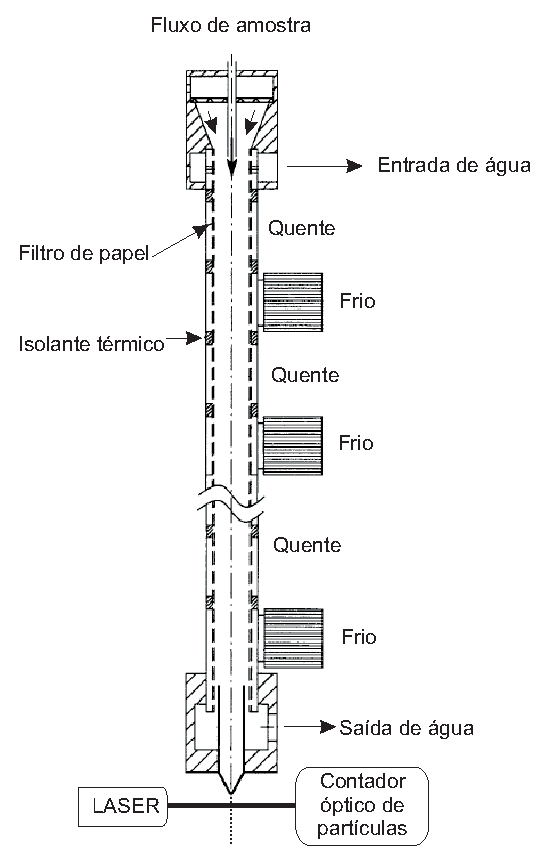
\includegraphics[scale=0.8]{eps/caltech.eps}\\
\end{center}
\caption{\label{caltech}\hspace{-0.1em} diagrama esquem\'{a}tico da c\^{a}mara de difus\~{a}o de Chuang.}
\end{figure}

\newpage

%% ------------------------------------------------------------------------- %%

\section{CCNC-Peter}

O CCNC descrito nesta se\c{c}\~{a}o foi desenvolvido por Peter Otto e colaboradores
\cite{Otto} e foi apresentado em 2002. Trata-se de um CCNC de fluxo
cont\'{\i}nuo que implementa as t\'{e}cnicas de Fukuta e Saxena, sendo que utiliza tr\^{e}s
CCDs para a medida da concentra\c{c}\~{a}o dos CCNs em tr\^{e}s supersatura\c{c}\~{o}es diferentes. A c\^{a}mara \'{e} orientada verticalmente de modo que o ar amostrado flui de forma laminar entre as placas. Uma das placas \'{e} mantida usualmente a uma temperatura $T_c=20^o$C e outras tr\^{e}s mantidas nas temperaturas $T_{wi}$ abaixo de $T_c$. O controle das
supersatura\c{c}\~{o}es, a digitaliza\c{c}\~{a}o e o processamento digital das imagens
s\~{a}o realizadas por um microcomputador. Na Figura \ref{ccnc3e} \'{e} mostrado
um diagrama b\'{a}sico do sistema.  Este sistema apresenta um avan\c{c}o
significativo em rela\c{c}\~{a}o aos CCNCs anteriores, pois, j\'{a} incorpora
tecnologias baseadas em eletr\^{o}nica digital e processamento digital
de imagens, conferindo naturalmente ao sistema uma maior
estabilidade e exatid\~{a}o. Testes mostram uma boa correla\c{c}\~{a}o (99\%) entre este CCNC e um CPC em uma faixa de 10 at\'{e} 1000 part\'{\i}culas$ /\ $m$^3$.

Entretanto, \'{e} um sistema exigente, pois, \'{e} necess\'{a}ria a manuten\c{c}\~{a}o da  circula\c{c}\~{a}o de alguns mililitros por minuto de \'{a}gua nas placas. Al\'{e}m disto, essa \'{a}gua cont\'{e}m uma pequena quantidade( $7\times10^{-3} mol/l$) de timol, necess\'{a}rio para manter o interior da c\^{a}mara livre de fungos. Outro fator de complexidade \'{e} a necessidade de dois fluxos de ar limpo pr\'{o}ximos \`{a}s placas de difus\~{a}o de vapor para garantir que o ar amostrado se mantenha confinado na regi\~{a}o de m\'{a}xima supersatura\c{c}\~{a}o.



\begin{figure}[!hbt]
\begin{center}
\includegraphics[scale=1]{eps/ccnc3estagios.eps}\\
\end{center}
\caption{\label{ccnc3e}\hspace{-0.1em} diagrama esquem\'{a}tico da CCNC-Peter.}
\end{figure}
\newpage

%% ------------------------------------------------------------------------- %%

\section{O CCNC-MPI-Chemie}

H\'{a} um CCNC similar ao descrito por Lala e Jiusto \cite{Lala}, pertencente ao Instituto Max Plank para Qu\'{\i}mica que, como no caso do CCNC-Peter, utiliza tamb\'{e}m a tecnologia digital, sendo que, ao inv\'{e}s de tr\^{e}s CCDs, apenas uma \'{e} utilizada. A Figura \ref{ccncmainz} mostra o diagrama deste instrumento. Pelo fato deste CCNC utilizar uma c\^{a}mara est\'{a}tica, os seus problemas  s\~{a}o os mesmos encontrados no CCNC-WYO, no m\'{\i}nimo aqueles relacionados aos efeitos transit\'{o}rios j\'{a} descritos anteriormente.

O processamento digital de imagens, para contagem autom\'{a}tica do n\'{u}mero dos CCNs ativados, neste CCNC, considera a quantidade de objetos brancos e de \emph{pixels} brancos na imagem  para calcular a quantidade de got\'{\i}culas \cite{Frank}. Corre\c{c}\~{o}es emp\'{\i}ricas s\~{a}o utilizadas para os casos de concentra\c{c}\~{o}es mais elevadas, onde o efeito de sobreposi\c{c}\~{o}es de got\'{\i}culas \'{e} mais acentuado. Essa t\'{e}cnica apresentou resultados razo\'{a}veis para  concentra\c{c}\~{o}es  abaixo de 600 cm$^{-3}$, mas para concentra\c{c}\~{o}es mais altas, encontradas em muitas situa\c{c}\~{o}es de interesse, os resultados mostram uma subestima\c{c}\~{a}o sistem\'{a}tica do n\'{u}mero de part\'{\i}culas ativadas \cite{Frank,Rose}.


\begin{figure}[!hbt]
\begin{center}
\includegraphics[scale=0.9]{eps/ccnc_mainz.eps}\\
\end{center}
\caption{\label{ccncmainz}\hspace{-0.1em} diagrama esquem\'{a}tico do CCNC do Max Plank Institute.}
\end{figure}
